\documentclass{article}

\usepackage{url,graphicx,tabularx,array,geometry, hyperref}
\usepackage{listings}
\usepackage{fullpage}
\usepackage{fancyvrb}
\usepackage{framed}
\usepackage{lastpage}
\usepackage{fancyhdr}

\renewcommand{\headrulewidth}{0pt}
\setcounter{secnumdepth}{0}

\setlength{\parskip}{1ex} %--skip lines between paragraphs
\setlength{\parindent}{0pt} %--don't indent paragraphs
\setlength{\headheight}{15.2pt}

\pagestyle{fancy}

\renewcommand{\headrulewidth}{0pt}
\lhead{  }
\lfoot{Lab 6: TCP Congestion Control}
\rfoot{page \thepage\ of \pageref{LastPage}}

\renewcommand{\familydefault}{\sfdefault}
\begin{document}

\begin{titlepage}
\begin{center}
\textsc{\huge \bfseries Advanced Networking 2020}\\[1.5cm]
\textsc{\large Lab \#1: TCP Congestion Control}\\[1.5cm]
\textsc{\huge Report}\\[1.5cm]
\textsc{\huge \bfseries GROUP: 5}\\[1.5cm]
\textsc{\large{\textbf{Authors:}\\ Arnold Buntsma, arnold.buntsma@os3.nl\\ Sean Liao, sean.liao@os3.nl}}

\textsc{\large University of Amsterdam}
\end{center}
\end{titlepage}

% https://inst.eecs.berkeley.edu/~ee122/fa05/projects/Project2/SACKRENEVEGAS.pdf
% http://intronetworks.cs.luc.edu/current/html/reno.html



% ./waf --run tcp-variants-comparison --command-template="%s --tracing=1 --pcap_tracing=1 --duration=400 --sack=true --prefix_name=TcpNewReno --transport_prot=TcpNewReno"

\subsection{Q1.1 Plot a graph showing SSTH versus time from 0.0s to
400.0s, 0.0s to 50.0s, then discuss}

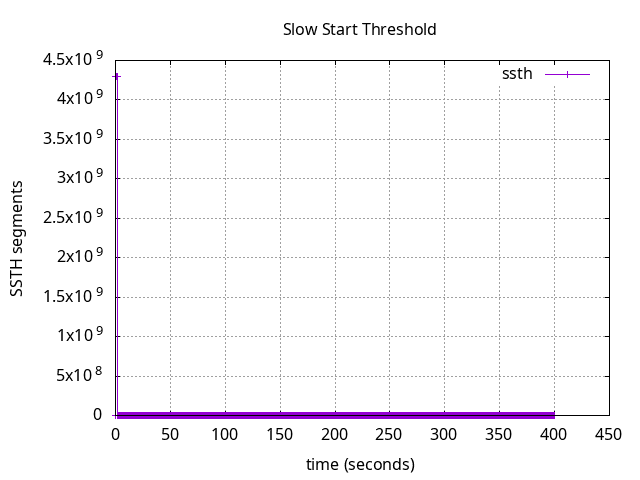
\includegraphics[scale=0.5]{plots/lab1-group5-task1-question1.1.png}
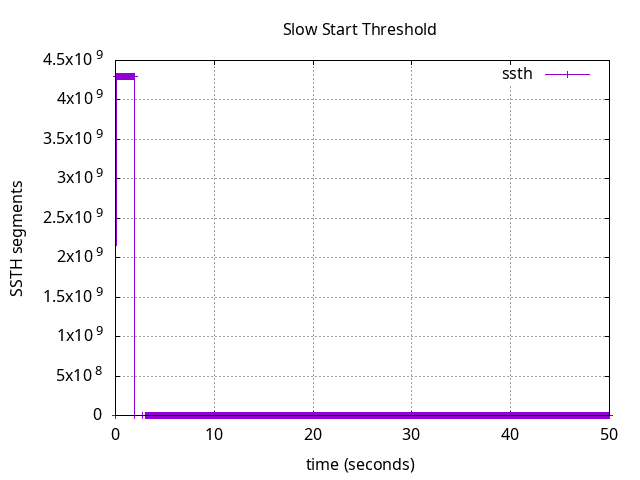
\includegraphics[scale=0.5]{plots/lab1-group5-task1-question1.1-xrange-0-50.png}
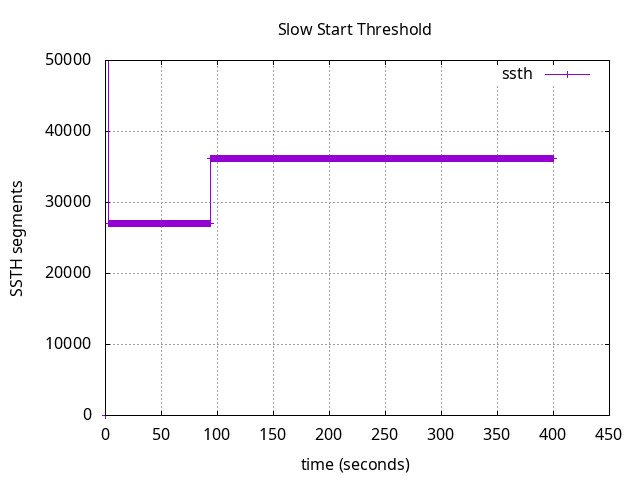
\includegraphics[scale=0.5]{plots/lab1-group5-task1-question1.1-yrange-0-50000.png}
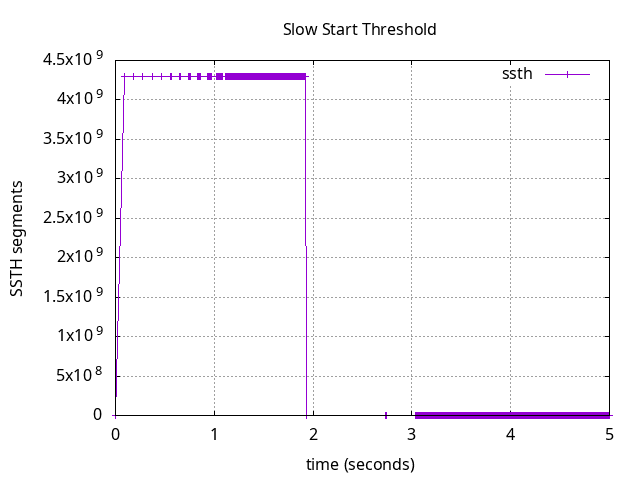
\includegraphics[scale=0.5]{plots/lab1-group5-task1-question1.1-xrange-0-5.png}

From RFC 2001\footnote{https://tools.ietf.org/html/rfc2001}: "Initialization for a given connection sets cwnd to one segment and ssthresh to 65535 bytes." This can be seen in the graph that the ssth is set to 65535 bytes. That explains the spike in the beginning of the graph. Then congestion occurs and the ssth is set to half of the current cwnd. This happens twice, setting SSTH low enough. SSTH is adjusted once more when congestion control hits its first congestion event during congestion avoidance. This threshold remains to the end as the test environment is stable.

\subsection{Q1.2 Plot a graph showing INFLIGHT versus time from 0.0s to
400.0s and discuss.}

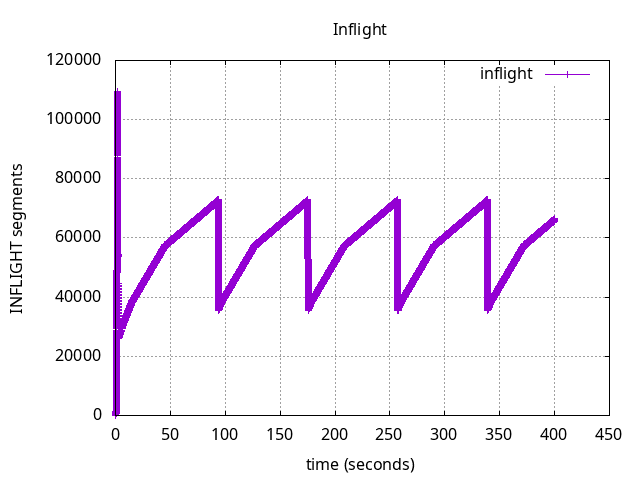
\includegraphics[scale=0.5]{plots/lab1-group5-task1-question1.2.png}

It matches the cwnd graph but slightly delayed, as expected, since it takes time for inflights to complete and the new window to take effect. This is because the amount of segments inflight should be similar to the congestion window if the buffer of the receiving end is big enough. It grows first rapidly because of slow start. Then congestion events halve the cwnd and it goes into fast recovery, then when the ssth is met it goes into congestion avoidance until another congestion happens and then the cylce of fast recovery etc. starts again.


\subsection{Q1.3 Plot a graph showing CWND versus time from 0.0s to 400.0 and discuss.}

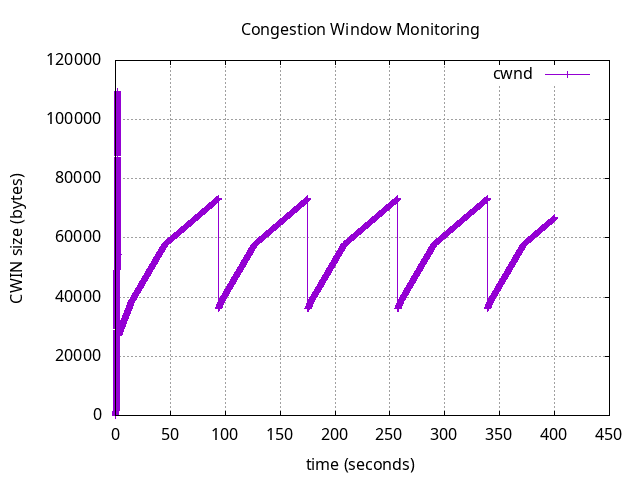
\includegraphics[scale=0.5]{plots/lab1-group5-task1-question1.3.png}
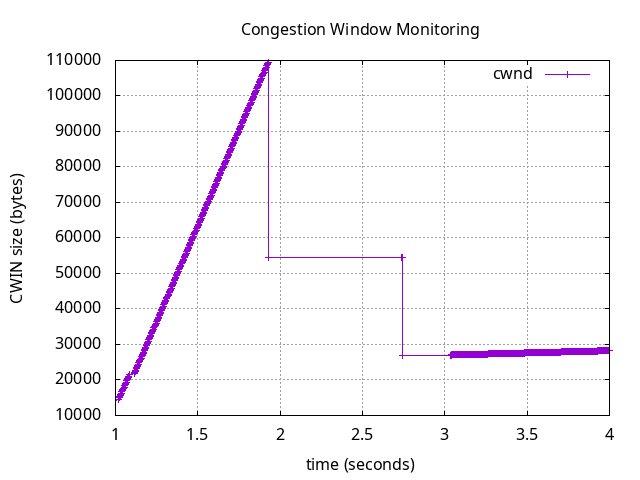
\includegraphics[scale=0.5]{plots/lab1-group5-task1-question1.3-xrange-1-4.png}

As expected, the congestion window grows rapidly during initial slow start. Congestion events then push the window into a cycle of fast recovery and congestion avoidance. With NewReno, Fast Retransmit means the window is never reset to 1, maintaining a full pipeline. It is notable that the network the congestion point is stable across cycles, reflecting the fact that there is nothing else on the network so TCP congestion is fighting itself.

\subsection{Q1.4 P Find the points where the slow-start, congestion-avoidance, fast retransmit/fast recovery states begin. When analyze the CWND changes use the layout of Table 1. This will allow you to identify where state-change points occurred and fill in following fields in the table below: the time, CWND before and after change, inFlight, SSThreshold, the new state, and the event that caused the change. Provide also the initial states.}

\begin{table}[h]
\begin{tabular}{|l|l|l|l|l|l|l|}
\hline
Event           & Time (s)  & Current CWND (bytes) & Next CWND(bytes) & FlightSize & SSThrehold & New State  \\ \hline
init	& 0	        & 0	        & 340	& 0         & 4294967295    & slow start \\ \hline
3x dup ACK	& 1.93197	& 109480	& 54400	& 108800	& 54400	& fast recovery \\ \hline
ACK	& 1.93197	& 54400	& 54402	& 108800	& 54400	& congestion avoidance \\ \hline
3x dup ACK	& 2.74046	& 54402	& 27030	& 54060	& 27030	& fast recovery \\ \hline
ACK	& 2.74046	& 27030	& 27034	& 54060	& 27030	& congestion avoidance \\ \hline
3x dup ACK	& 93.5542	& 73207	& 36210	& 72420	& 36210	& fast recovery \\ \hline
ACK	& 93.5542	& 36210	& 36213	& 72420	& 36210	& congestion avoidance \\ \hline
3x dup ACK	& 175.257	& 73207	& 36210	& 72420	& 36210	& fast recovery \\ \hline
ACK	& 175.262	& 36210	& 36213	& 72420	& 36210	& congestion avoidance \\ \hline
3x dup ACK	& 256.965	& 73207	& 36210	& 72420	& 36210	& fast recovery \\ \hline
ACK	& 256.97	& 36210	& 36213	& 72420	& 36210	& congestion avoidance \\ \hline
3x dup ACK	& 338.672	& 73207	& 36210	& 72420	& 36210	& fast recovery \\ \hline
ACK	& 338.677	& 36210	& 36213	& 72420	& 36210	& congestion avoidance \\ \hline

\end{tabular}
\caption{Tcp Congestion Control}
\label{tab:scenario1}
\end{table}

It wasn't really clear what triggered an event to be recorded and when the logs were taken (before, during, after an event). The low timer resolution and non matching records across logs did not help. The pcaps also had back checksums which hindered analysis.

\subsection{Q1.5 Explain what SACK does. Replicate scenario 1 of the simulation with SACK Off:  \textbf{Sack=0}. Answer questions and compare the two results.}
SACK is selective acknowledgement of segments instead of the standard cumulative acknowledgements. This works by putting in a options field that a endpoint got for example segments 1, 2 \& 4 correctly. Then the sending host knows it has to resend segment 3. This option has to be enabled by both hosts and negotiated in the connection setup. \footnote{https://packetlife.net/blog/2010/jun/17/tcp-selective-acknowledgments-sack/} 
% ./waf --run tcp-variants-comparison --command-template="%s --tracing=1 --pcap_tracing=1 --duration=400 --sack=false --prefix_name=TcpNewReno --transport_prot=TcpNewReno"


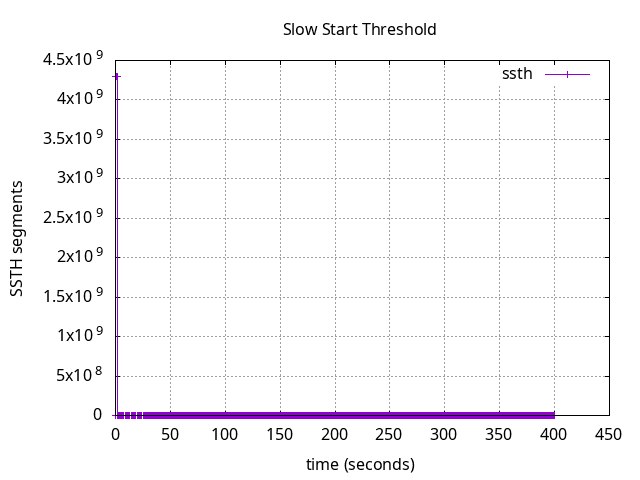
\includegraphics[scale=0.5]{plots/lab1-group5-task1-experimentA-question1.1.png}
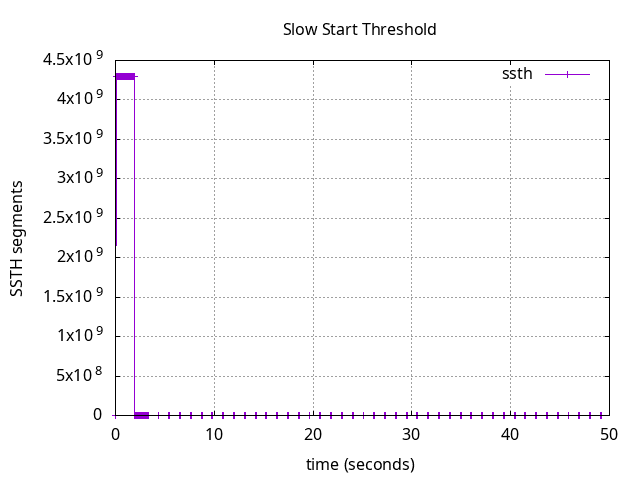
\includegraphics[scale=0.5]{plots/lab1-group5-task1-experimentA-question1.1-xrange-0-50.png}
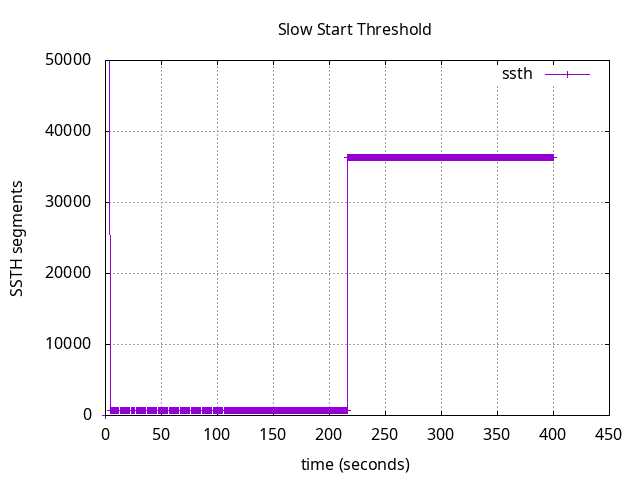
\includegraphics[scale=0.5]{plots/lab1-group5-task1-experimentA-question1.1-yrange-0-50000.png}

For the ssth there is no change in the results which is to be expected. The ssth only changes if there is a timeout or a triple duplicate ack and these are not different from the first experiment. It is raised at the same point, after the first congestion cycle.

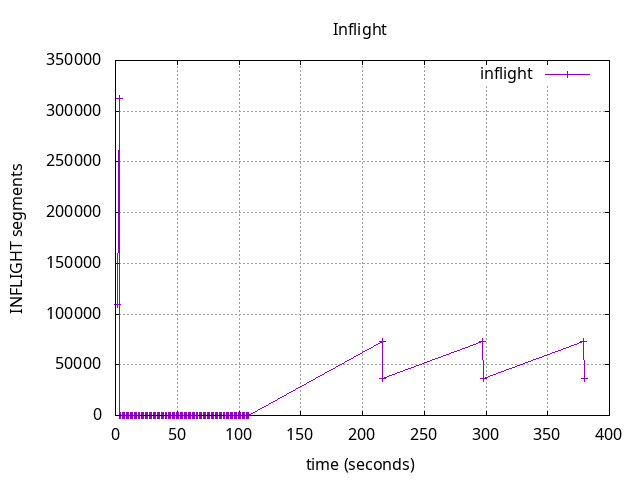
\includegraphics[scale=0.5]{plots/lab1-group5-task1-experimentA-question1.2.png}

Inflight is related to the congestion window but follows a different curve. The congestion cycles are visible but much less pronounces than with SACK on. The amount of inflight is comparable to when SACK is on. Only the initial spike is higher then when SACK is on.

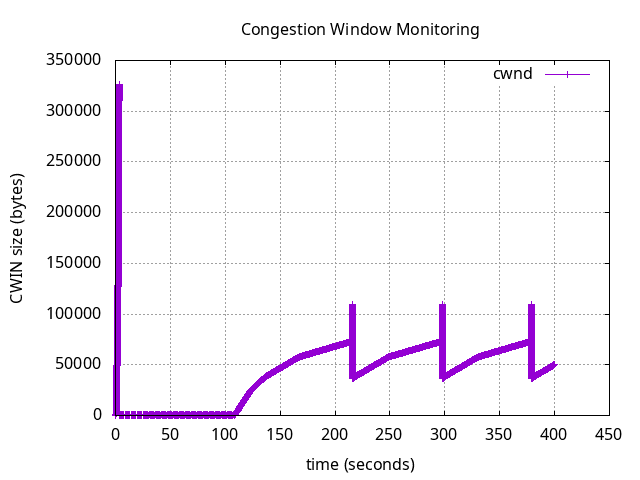
\includegraphics[scale=0.5]{plots/lab1-group5-task1-experimentA-question1.3.png}
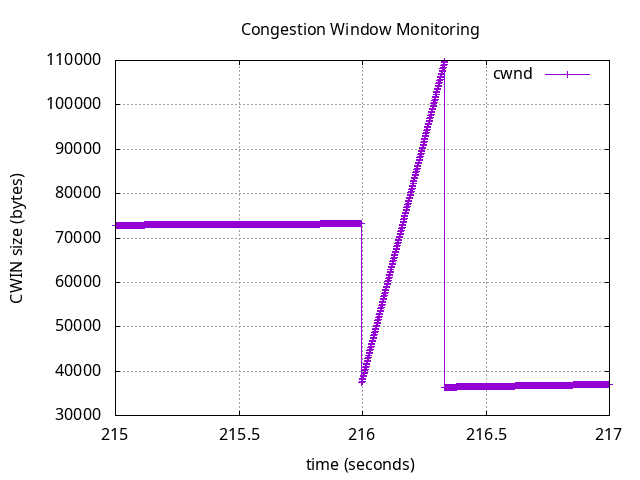
\includegraphics[scale=0.5]{plots/lab1-group5-task1-experimentA-question1.3-xrange-215-217.png}

It appears that after the initial flood from slow start, it times out, and remains suppressed for a long time for unknown reasons (lots of timeouts?). It is also unclear what triggers the eventual increase in  the congestion window.  During the congestion cycles, duplicate ACKs trigger fast recovery, without SACK to only resend the missing piece, fast recovery is highly aggressive in resending  packets before returning back to congestion avoidance with a lower window.

\begin{table}[h]
\begin{tabular}{|l|l|l|l|l|l|l|}
\hline
Event           & Time (s)  & Current CWND (bytes) & Next CWND(bytes) & FlightSize & SSThrehold & New State  \\ \hline
init	& 0	        & 0             & 340	        & 0	        & 4294967295    & slow start \\ \hline
timeout	& 3.26916	& 326570	& 340	        & 312800        & 156400	& fast recovery \\ \hline
ACK	& 4.30286	& 680	        & 340	        & 0	        & 680	        & congestion avoidance \\ \hline
3x dup ACK	& 215.997	& 73207	        & 37400	        & 72760	        & 36380	        & fast recovery \\ \hline
ACK	& 216.333	& 109820	& 36380	        & 36040         & 36380	        & congestion avoidance \\ \hline
3x dup ACK& 297.52	& 73207	        & 37400	        & 72760	        & 36380         & fast recovery \\ \hline
ACK	& 297.861	& 109820	& 36380	        & 36040         & 36380	        & congestion avoidance \\ \hline
3x dup ACK	& 379.049	& 73207	        & 37400	        & 72760         & 36380	        & fast recovery \\ \hline
ACK	& 379.389	& 109820	& 36380	        & 36040         & 36380	        & congestion avoidance \\ \hline
\end{tabular}
\caption{Tcp Congestion Control}
\label{tab:scenario1}
\end{table}

The table looks almost the same as Q1.4 even though the graphs look different due to the different behaviour of fast recovery. The fast recovery phase is longer as without SACK it has more things to resend. 


\subsection{Q1.6 Replicate scenario 1 of the simulation and answer the questions: \textbf{Packet loss of 4\%, Sack=0 and transfer duration of 400sec}. Answer the questions and explain the results.
}

\textbf{SSTH}

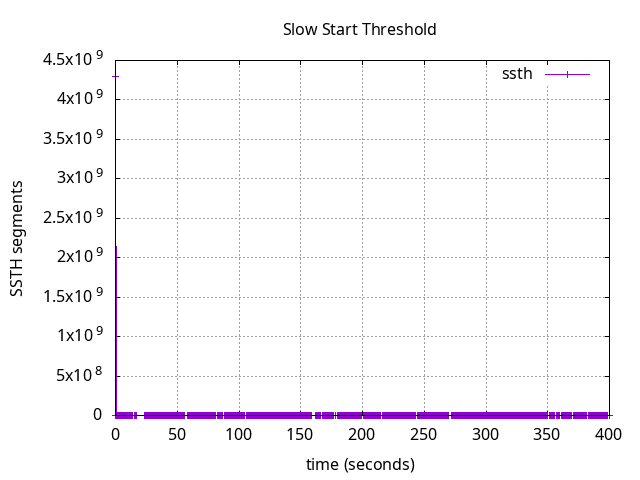
\includegraphics[scale=0.5]{plots/lab1-group5-task1-experimentB-question1.1.png}
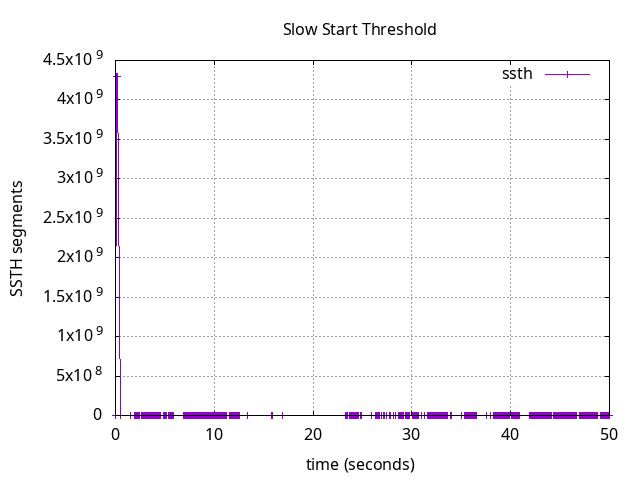
\includegraphics[scale=0.5]{plots/lab1-group5-task1-experimentB-question1.1-xrange-0-50.png}
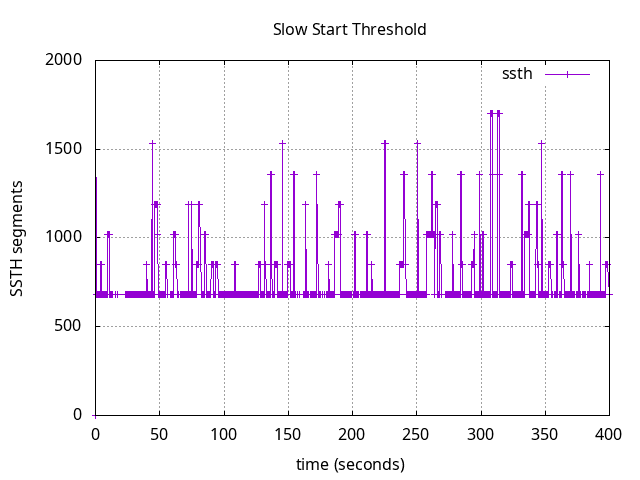
\includegraphics[scale=0.5]{plots/lab1-group5-task1-experimentB-question1.1-yrange-0-2000.png}
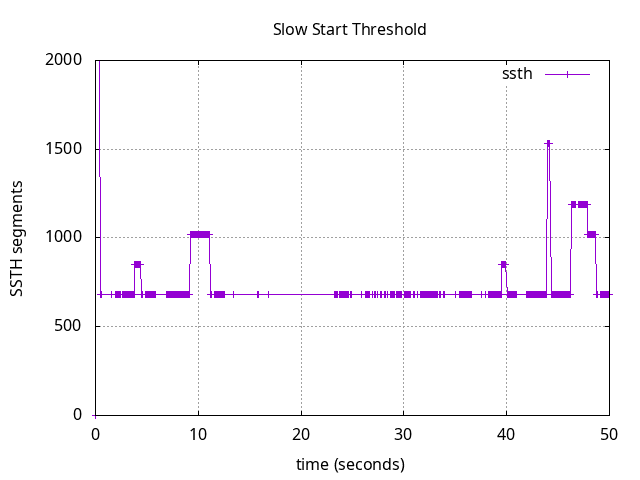
\includegraphics[scale=0.5]{plots/lab1-group5-task1-experimentB-question1.1-xrange-0-50-yrange-0-2000.png}

As you can see the ssth drops very quickly because there is a packet loss of 4\%. This will lead to more duplicate acks and thus reduce the ssth and keep it low. Occasionally, longer periods of uninterrupted transmissions allow for ssth to be set at higher levels, but this is quickly returned to baseline when more frequent packet



% ./waf --run tcp-variants-comparison --command-template="%s --tracing=1 --pcap_tracing=1 --duration=400 --sack=false --error_p=0.04 --prefix_name=TcpNewReno --transport_prot=TcpNewReno"
\textbf{INFLIGHT}

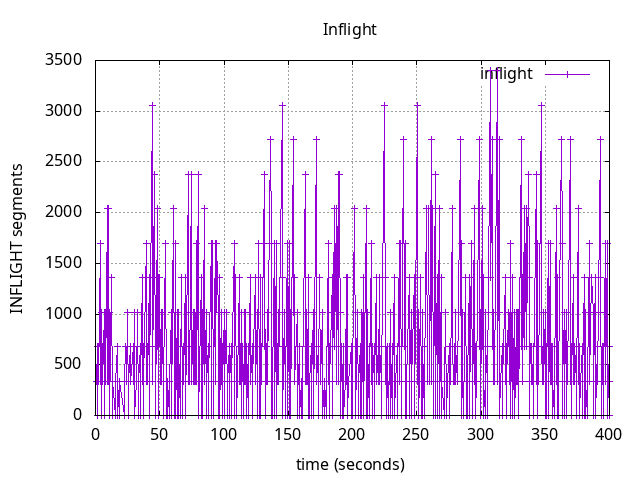
\includegraphics[scale=0.5]{plots/lab1-group5-task1-experimentB-question1.2.png}

The inflight correlates a bit with the cwnd however because of the packet loss are there more packets inflight that do not arrive which will decrease the cwnd. But overall the two correlate quite good. If there are many segments in flight the cwnd is also larger. The reason this graph is all over the place is because of the packet loss and therefore changing the cwnd every time. 

\textbf{CWND}

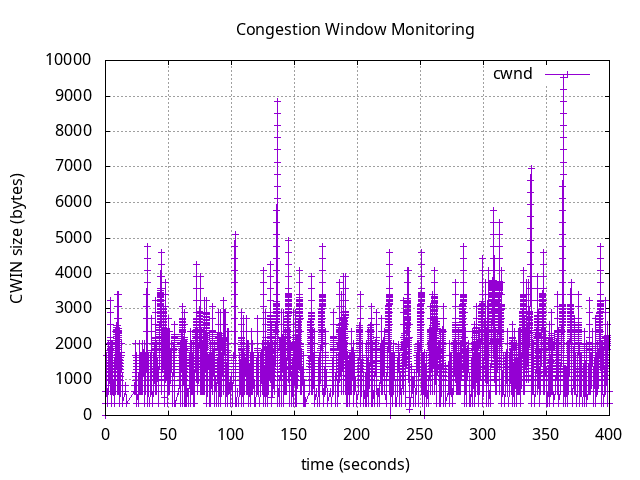
\includegraphics[scale=0.5]{plots/lab1-group5-task1-experimentB-question1.3.png}
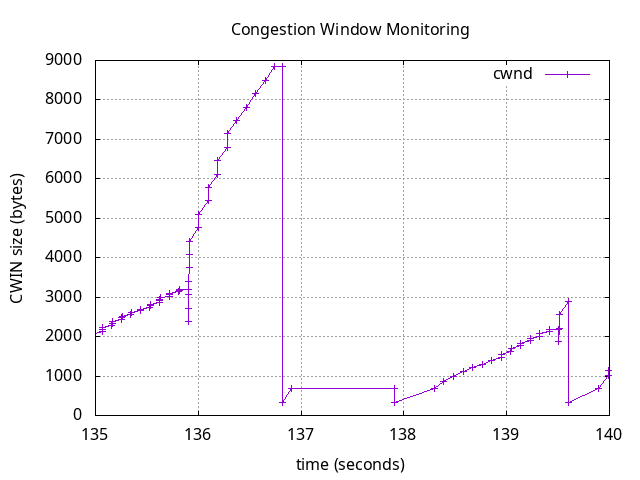
\includegraphics[scale=0.5]{plots/lab1-group5-task1-experimentB-question1.3-xrange-135-140.png}

The cwnd correlates with the inflight. This is logical because if the cwnd is bigger, there can be more segments inflight. Similar to the inflight reason that this graph seems to be all over the place, is because of the packet loss. When that happens the cwnd decreases. 

The 4\% packet loss triggers the congestion control much earlier and much more often, resulting in multiple state changes in short periods of time, but from the zoomed in view of cwnd, even though each cycle is shorter, it still follows the same patterns as before, just with different values as the size of cwnd differs each time a loss occurs.

\subsection{Q1.7  Replicate scenario 1 of the simulation:  \textbf{Delay of 300 ms, Sack=true and transfer duration of 400sec}. Answer the questions and explain the results.}

% ./waf --run tcp-variants-comparison --command-template="%s --tracing=1 --pcap_tracing=1 --duration=400 --sack=true --delay=300ms --prefix_name=TcpNewReno --transport_prot=TcpNewReno"


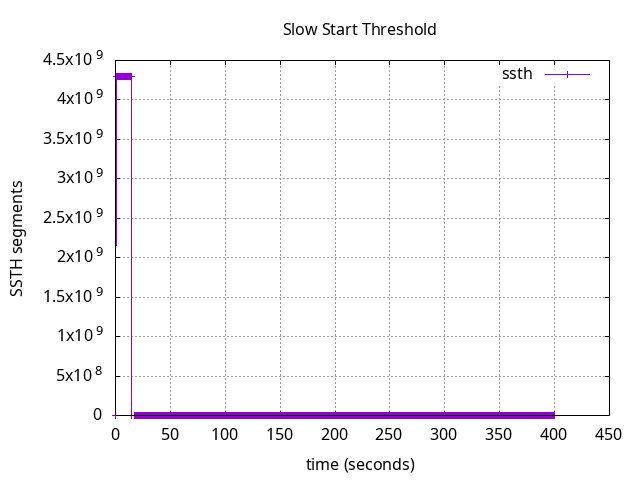
\includegraphics[scale=0.5]{plots/lab1-group5-task1-experimentC-question1.1.png}
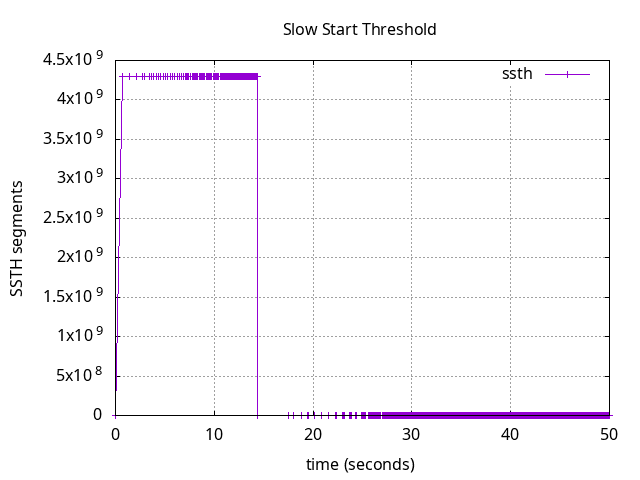
\includegraphics[scale=0.5]{plots/lab1-group5-task1-experimentC-question1.1-xrange-0-50.png}
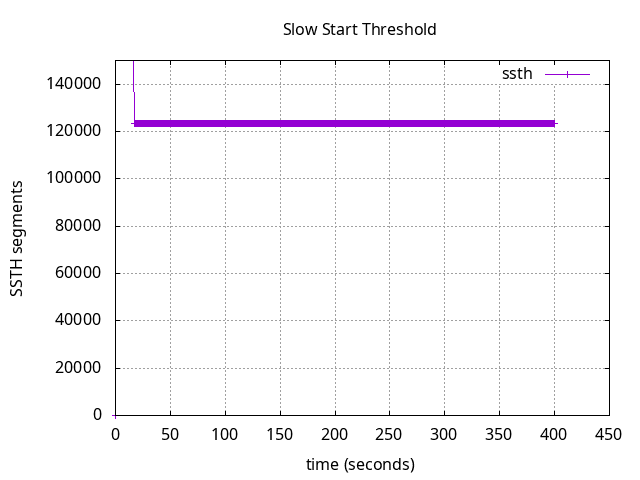
\includegraphics[scale=0.5]{plots/lab1-group5-task1-experimentC-question1.1-yrange-0-150000.png}
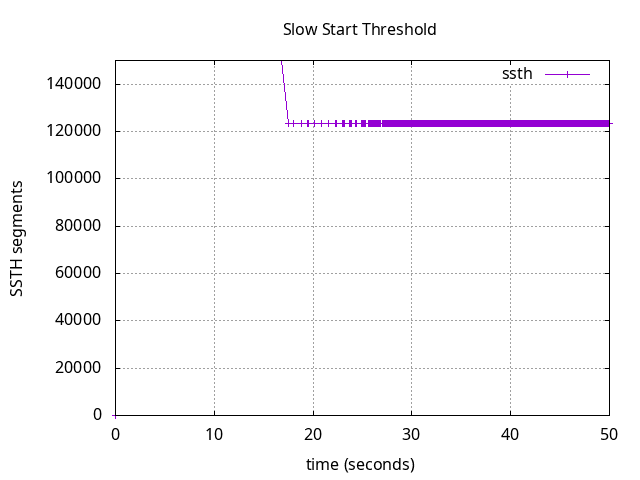
\includegraphics[scale=0.5]{plots/lab1-group5-task1-experimentC-question1.1-xrange-0-50-yrange-0-150000.png}

The slow start threshold looks similar to the results in Q1.1 but stretched out. This is expected considering every step in the TCP congestion control state machine requires a rountrip time. Without hitting the first congestion cycle, ssth is not raised to a higher level.

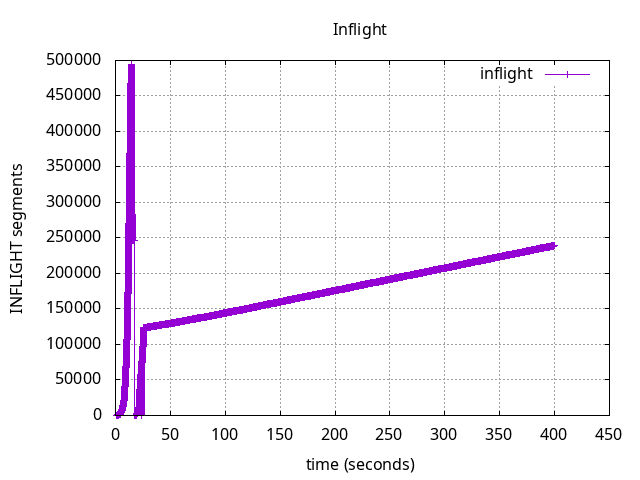
\includegraphics[scale=0.5]{plots/lab1-group5-task1-experimentC-question1.2.png}

Again, inflight closely matches the congestion window like with the other experiments. This has the same explanation as the other experiments.

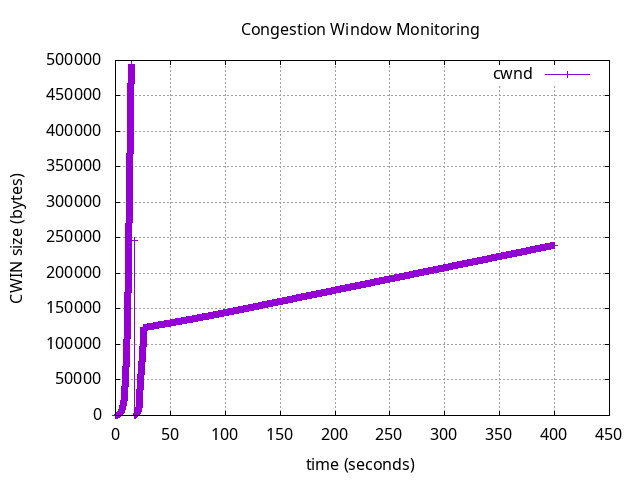
\includegraphics[scale=0.5]{plots/lab1-group5-task1-experimentC-question1.3.png}
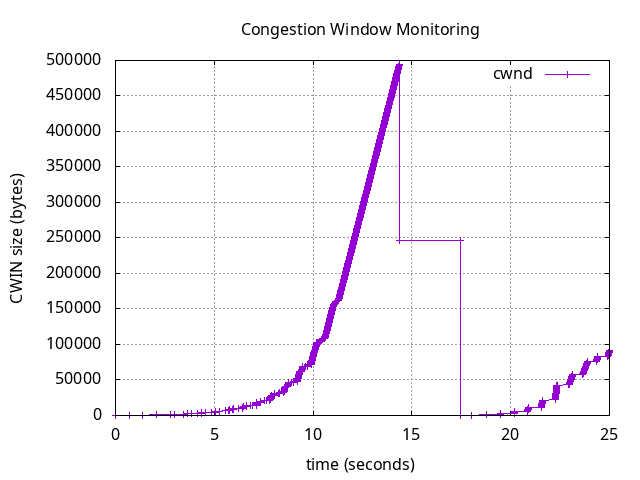
\includegraphics[scale=0.5]{plots/lab1-group5-task1-experimentC-question1.3-xrange-0-25.png}

Here the longer roundtrip time results in a timeout instead of just duplicate acks, resulting in slow start starting up again after the initial probe. The second time, ssth is already set so it successfully transitions into the congestion avoidance phase. The testing duration was not long enough for tcp to hit its first cycle.

\begin{table}[h]
\begin{tabular}{|l|l|l|l|l|l|l|}
\hline
Event           & Time (s)  & Current CWND (bytes) & Next CWND(bytes) & FlightSize & SSThrehold & New State  \\ \hline
init	& 0	& 0	& 340	& 0	& 4294967295 &slow start \\ \hline
3x dup ACK	& 14.3792	& 495040	& 247180	& 494360	& 247180	& fast recovery \\ \hline
timeout	& 17.4635	& 247180	& 340	& 0	& 123590	& slow start \\ \hline
cwnd=ssth	& 25.2946	& 123760	& 123761	& 122740	& 123590	& congestion avoidance \\ \hline

\end{tabular}
\caption{Tcp Congestion Control}
\label{tab:scenario1}
\end{table}



\subsection{Q2}

No screenshots, we provided the graphs.


\subsection{Q2.1 Plot a graph showing the CWND and ssthresh versus time with all the data you get. These two metrics are in one graph.}

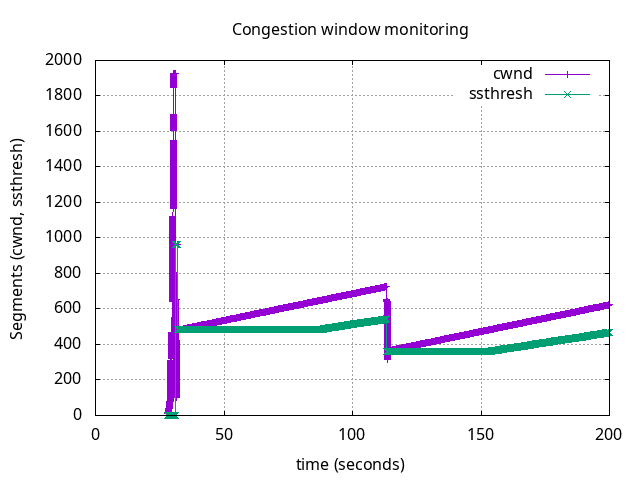
\includegraphics[scale=0.5]{plots/lab1-group5-task2-question2.1.png}
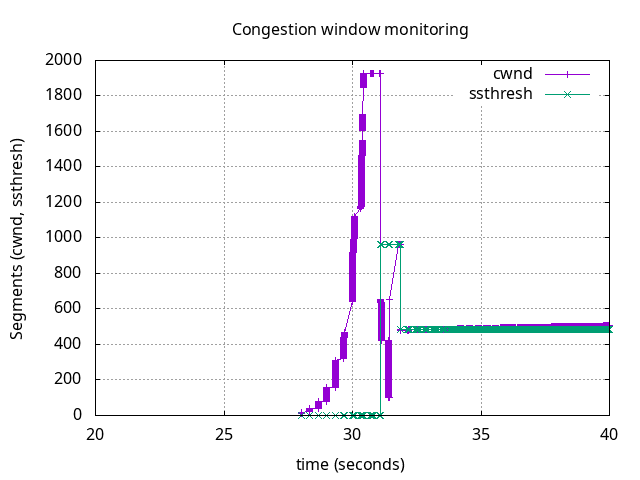
\includegraphics[scale=0.5]{plots/lab1-group5-task2-question2.1-xrange-20-40.png}

\subsection{Q2.2 Briefly discuss the changing process, motivate your answer.}

The process is mostly the same as NewReno explored in question 1, initial probing, timeout, slow start again, settle in to a stable cycle without interruption. It is unclear why ssth changes before a congestion event.

\subsection{Q2.3 Plot a graph showing CWND versus time with all the data you get.}

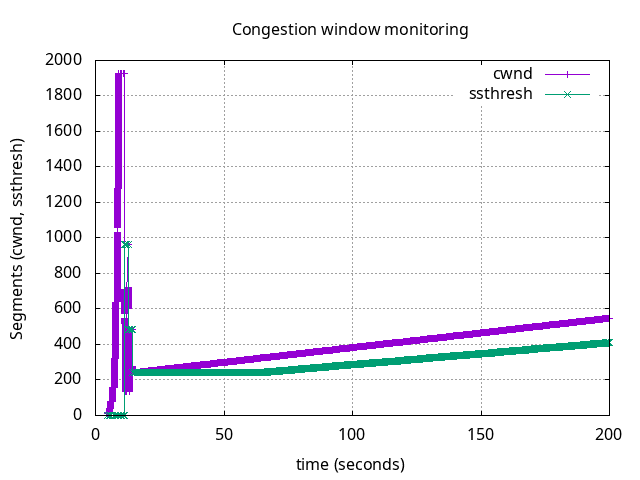
\includegraphics[scale=0.5]{plots/lab1-group5-task2-question2.3.png}
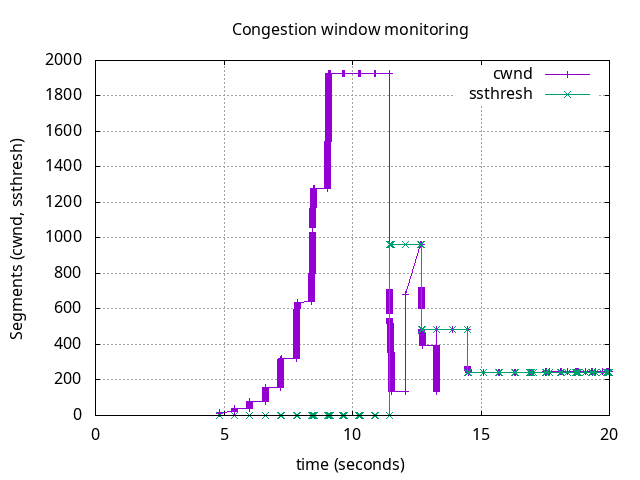
\includegraphics[scale=0.5]{plots/lab1-group5-task2-question2.3-xrange-0-20.png}

\subsection{Q2.4 Compare this graph with the one from Q2.1, show the difference between these two
graphs and discuss why these occur}

With a much higher latency, the order of events is similar to Q2.1, but slower. Also it appears that the higher latency is more prone to triggering a timeout, resulting in a lower starting point for the congestion control algorithm.

\subsection{Q2.5 Plot a graph showing CWND and ssthresh versus time with all the data you get.}

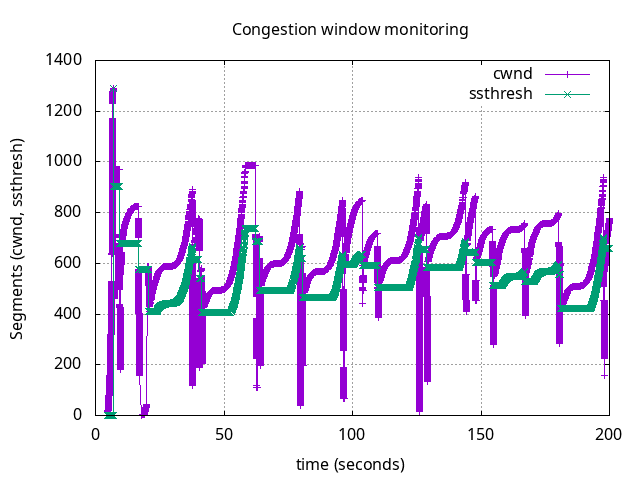
\includegraphics[scale=0.5]{plots/lab1-group5-task2-question2.5.png}
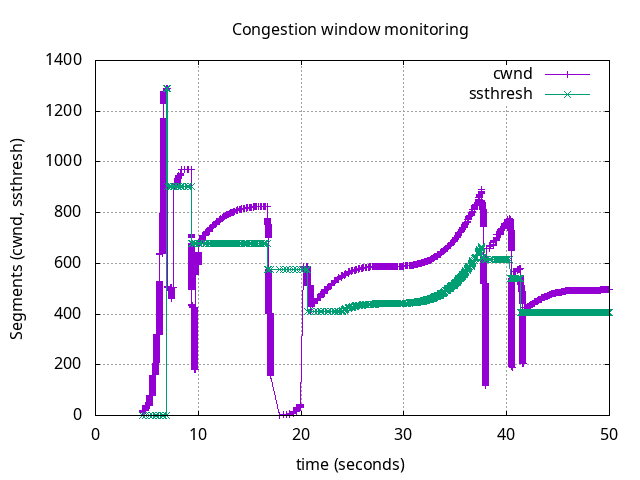
\includegraphics[scale=0.5]{plots/lab1-group5-task2-question2.5-xrange-0-50.png}

\subsection{Q2.6 Compare this graph with the graph of Q2.1, and discuss the (major) differences.}

The cubic curve obviously looks different from reno. They appear to have a similar midpoint at around 600 bytes, but cubic has shorter cycles with greater variations in minimum and maximums. 

\subsection{Q2.7 Plot a graph showing CWND and ssthresh versus time with all the data you get.}

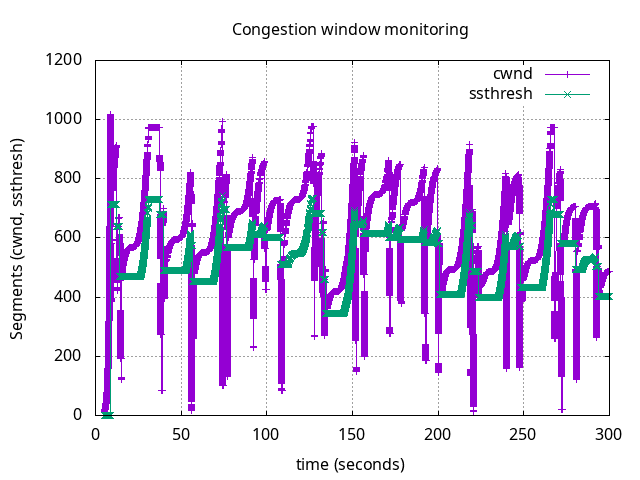
\includegraphics[scale=0.5]{plots/lab1-group5-task2-question2.7.png}
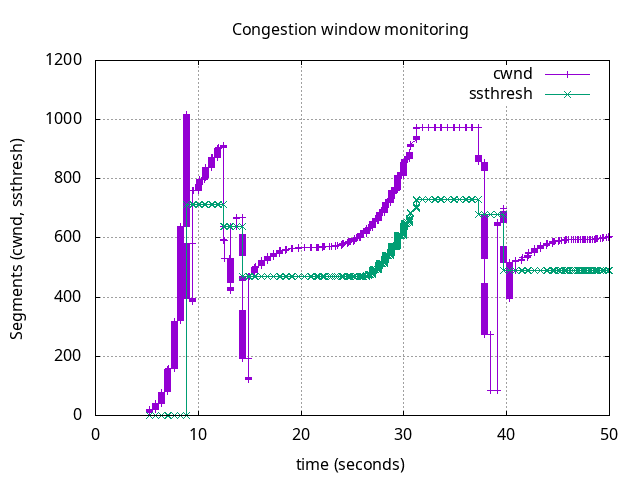
\includegraphics[scale=0.5]{plots/lab1-group5-task2-question2.7-xrange-0-50.png}

\subsection{Q2.8 Compare this graph with the graph of Q2.3 and discuss the (major) differences.}

With reno, higher latencies slowed down the growth of cwnd a lot during congestion avoidance, but with cubic, the aggressive growth at the start makes up for the longer latencies, resulting in similar cycles as it has in low latency environments

\end{document}
% Template for table used in Task 1
%
% \begin{table}
% \begin{tabular}{|c|p{25mm}|p{20mm}|c|c|}
% \hline Time (s)    & Current CWND (bytes)    & New CWND (bytes)    & New State    & Event \\
% \hline ...         &              &          &             & \\
% \hline ...         &              &          &             & \\
% \hline ...         &              &          &             & \\
% \hline ...         &              &          &             & \\
% \hline
% \end{tabular}
% \end{table}
